\documentclass[onecolumn, draftclsnofoot,10pt, compsoc]{IEEEtran}
\usepackage{graphicx}
\usepackage{url}
\usepackage{setspace}
\usepackage{geometry}
\usepackage{tabularx}
\geometry{textheight=9.5in, textwidth=7in}

\def \CapstoneTeamName{		    Comedy Robot Team}
\def \CapstoneTeamNumber{		43}
\def \GroupMemberOne{			Timothy Bui}
\def \GroupMemberTwo{			Yuhang (Tony) Chen}
\def \GroupMemberThree{			Brian Ozarowicz}
\def \GroupMemberFour{			Trevor Webster}
\def \CapstoneProjectName{		Building More Self-Aware\linebreak Everyday Robots}
\def \CapstoneSponsorCompany{	SHARE Lab}
\def \CapstoneSponsorPerson{	Dr. Naomi Fitter}

% Uncomment the appropriate line below so that the document type works
\def \DocType{	%Problem Statement
				Requirements Document
				%Technology Review
				%Design Document
				%Progress Report
				}
			
\newcommand{\NameSigPair}[1]{\par
\makebox[2.75in][r]{#1} \hfil 	\makebox[3.25in]{\makebox[2.25in]{\hrulefill} \hfill		\makebox[.75in]{\hrulefill}}
\par\vspace{-12pt} \textit{\tiny\noindent
\makebox[2.75in]{} \hfil		\makebox[3.25in]{\makebox[2.25in][r]{Signature} \hfill	\makebox[.75in][r]{Date}}}}
% If the document is not to be signed, uncomment the RENEWcommand below
\renewcommand{\NameSigPair}[1]{#1}

%%%%%%%%%%%%%%%%%%%%%%%%%%%%%%%%%%%%%%%
\begin{document}
\begin{titlepage}
    \pagenumbering{gobble}
    \begin{singlespace}
    	
\includegraphics[height=4cm]{coe_v_spot1}
        \hfill 
        % If you have a logo, use this includegraphics command to put it on the coversheet.
        %\includegraphics[height=4cm]{CompanyLogo}   
        \par\vspace{.2in}
        \centering
        \scshape{
            \huge CS Capstone \DocType \par
            %{\large\today}\par
            {\large Fall 2019}\par
            \vspace{.5in}
            \textbf{\Huge\CapstoneProjectName}\par
            \vfill
            {\large Prepared for}\par
            %\Huge \CapstoneSponsorCompany\par
            %\vspace{5pt}
            {\Large\NameSigPair{\CapstoneSponsorPerson}\par}
            {\large Prepared by }\par
            Group\CapstoneTeamNumber\par
            % comment out the line below this one if you do not wish to name your team
            \CapstoneTeamName\par 
            \vspace{5pt}
            {\Large
                \NameSigPair{\GroupMemberOne}\par
                \NameSigPair{\GroupMemberTwo}\par
                \NameSigPair{\GroupMemberThree}\par
                \NameSigPair{\GroupMemberFour}\par
            }
            \vspace{20pt}
        }
        \begin{abstract}
        	\noindent This document establishes the scope, goals, and requirements for the 'Building More Self-Aware Everyday Robots' Capstone project. The Capstone team will build on existing work started by the robot team to expand the use of machine learning over a full dataset of audio from past comedy performances. The learning will evaluate whether a particular joke was a hit or a bomb based on analysis of audience laughter. The results will be used to improve the real-time adaptive models the robot uses to respond to audience cues during a comedy performance. Accuracy of evaluating the audience response should be at least 85\% in order to match the performance of human evaluators.
        \end{abstract}
    \end{singlespace}
\end{titlepage}
\newpage
\pagenumbering{arabic}
\tableofcontents
% uncomment this (if applicable). Consider adding a page break.
%\listoffigures
%\listoftables
\clearpage

\section{Introduction}
This section describes the purpose and scope of the project and contains definitions of some of the terms referenced in this document.
\subsection{Purpose}
This document describes the requirements for the “Building More Self-Aware Everyday Robots” Capstone project. It establishes the goals for the project, deliverables and evaluation metrics, and lists potential stretch goals that could be included based on the success of the initial work.
\subsection{Scope}
The Capstone team will expand on previous work by the existing robot team (graduate students working under Dr. Fitter) by using machine learning on audio data from past comedy performances by the robot. The learning results will evaluate how well each joke was received based on the audience's reaction, determining it to be either a success, a bomb, or a mixed reaction, and be used to update the real-time adaptive models of the robot used during its comedy performances.
\subsection{Terms and Definitions}
\begin{itemize}	
\item Bomb: A joke that elicits negative or no reaction from the audience
\item Hit: A joke that elicits near-unanimous positive reaction from the audience
\item Machine Learning: Using patterns in data to automate analytical decision making without needing human input
\item NAO Robot: (pronounced now), an autonomous, programmable humanoid robot [1]
\item Python: an interpreted, general-purpose programming language
\item SciKit: a Python library for performing software machine learning [2]
\end{itemize}
\subsection{References}
[1] \textit{SoftBank Robotics NAOqi Documentation Center,} Accessed on: Oct 25, 2019. [Online] Available: http://doc.aldebaran.com\par
\noindent [2] \textit{Documentation of scikit-learn 0.21.3,} Accessed on: Oct 25, 2019. [Online] Available: https://scikit-learn.org/stable/\par
documentation.html
\subsection{Overview}
The rest of this document details the deliverable goals of this project and details of the tasks that comprise the work toward those goals.

\section{Overall Description}
This section describes the perspective and functions of the project and constraints and assumptions affecting the work that will be done.
\subsection{Perspective}
The purpose of this project is to increase successful human-robot interactions with a robotic stand-up comedian by improving the robot's real-time analysis of audience responses to determine whether a joke was a hit or a bomb. The result of this analysis can be used to make an appropriate follow-up remark based on the joke's reception, improving the dynamics of the robot's connection with its audience.
\subsection{Functions}
The NAO robot is capable of telling jokes using speakers, making basic body motions to accentuate the jokes, and listen to the audience's response to jokes. The existing team has already given it the capabilities for analysis of audience responses.\par
\vspace{.4cm}
\noindent Audience laughter is identified from other noise using audio frequency. The existing team has performed machine learning on some of this data using classifiers to identify hit jokes from bombs. The work of the Capstone team is to extend this approach by performing machine learning over the full dataset of past performances, improving the ability to autonomously determine how well a joke was received. This evaluation is used by the robot to decide when a follow-up remark about the joke is appropriate, so improved accuracy of the machine learning will lead to improvement in the robot's real-time adaptation during its performances.
\subsection{User Characteristics}
The users of our work will be Dr. Fitter and the existing robot team. This work builds on initial progress they made in using machine learning implemented in Python with SciKit for the analysis of joke performance.
\subsection{Constraints}
1. NAO Robot Hardware
\begin{itemize}	
\item Microphone audio quality affects how effective the analysis can be because the evaluation is done using the raw audio of audience reactions
\item Processing speed capabilities on the robot could affect what methods are able to be implemented for doing real-time analysis
\item The robot is currently unable to listen for audience reactions mid-joke, it only begins sensing feedback when the delivery concludes
\end{itemize}
2. Time
\begin{itemize}	
\item Background research and gaining familiarity with how the machine learning is performed using SciKit may impact the start of implementation
\item Project timeframe may limit opportunities for observation of the robot modifications in practice
\end{itemize}
\subsection{Assumptions and Dependencies}
We are assuming the machine learning pipeline initially designed by the existing robot team is successful for analyzing their dataset and our task is to extend that process over the full set of performance data, adjusting learning methods as necessary to improve success rates but not needing to develop a new process for performing the learning over the dataset. The work is dependent on the audio recordings being of a high enough quality for analysis to be possible.

\section{Specific Requirements}
This section describes the primary project goals expected as deliverables, the metric for evaluating goal success, and some potential stretch goals that could be included, time and progress permitting. It concludes with a Gantt chart of the expected project timeline.
\subsection{Interfaces}
The robot uses a microphone to sense audience reactions used for performance evaluation and to record the audio used for the machine learning analysis. Analysis of the dataset is done using bash scripts to extract features from the audio files and Python scripts to perform the classifier and validation techniques that have been implemented.
\subsection{Functional Requirements}
The machine learning on the past performance dataset should use classifiers to evaluate a joke as a hit (near-unanimous positive reaction), a bomb (negative or no reaction), or a mixed reaction based on analysis of audience laughter. The robot's real-time adaptive models use evaluation of the audience's reaction to a joke to dynamically adjust its performance by potentially adding a remark about how the joke was received before continuing on. To further enhance the machine learning capabilities of the robot more features will need to be extracted, classified, and added.\par
\vspace{.4cm}
\noindent The robot will also need to have the ability to analyze the audience while telling a joke to allow for more flexibility in joke delivery. To assist with this functionality there will need to be a way for the robot to reduce ambient noise to prevent picking up on false positives and improve its audience detection accuracy.
\subsection{Performance Requirements}
The accuracy of the automated joke evaluation (as a hit, a bomb, or mixed) must be 85\% or greater, to match the observed accuracy rate of human evaluation of joke reception. This accuracy is measured and calibrated by comparing the results from the robot with manually classified and tagged results from humans. There are multiple people categorizing the same results; in the even of conflicting opinions the average is taken. The real-time analysis methods that are implemented on the robot must be able to be run without interfering with the timing of the comedy performance.\par
\vspace{.4cm}
\noindent The robot's behavior should also be adjusted to introduce the ability to detect audience reaction mid-joke. Currently the robot cannot hear the audience while telling a joke, it only begins listening after the delivery is completed.
\subsection{Stretch Goal}
If progress on the stated project goals is made in a timely manner the team may also explore the possibility of adding a new feature to the robot's capabilities. The behavior would be modified to track audience reactions throughout a performance to see if they respond strongest to a particular type of joke or subject matter and make a remark about their tastes at the end of the performance.

\newpage
\subsection{Gantt Chart}
\begin{figure}[ht]
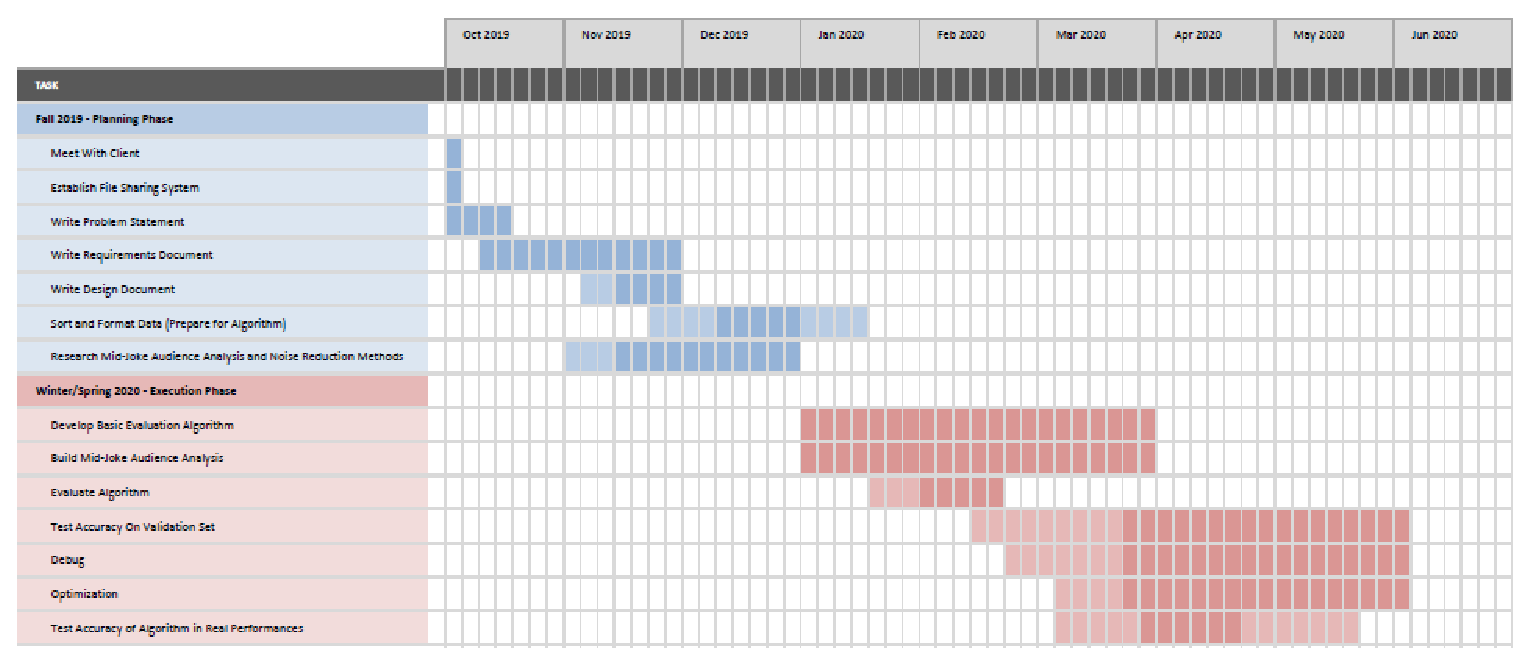
\includegraphics[width=\linewidth]{gantt.eps}
\caption{Estimated Project Timeline}
\end{figure}

\end{document}